\chapter{Implementation}
\label{impl}
The implementation chapter covers the technologies, techniques and patterns applied to this project.  Many of the contents were encountered were encountered during a summer placement at a technology company in Glasgow between levels 3 and 4.  

\section{Technologies Used and Discipline}
This section examines the technologies used in the implementation of the project and the discipline that was adhered to during development.

\subsection{Microsoft .NET Framework}
The Microsoft .\gls{net} framework is a platform for development, deployment and running of web services and applications \cite{whatIsDotNet}.  It provides a \gls{clr}, similar to the \gls{jvm} in Java  This project took advantage of \gls{asp}.\gls{net} \gls{mvc} 2.  

Microsoft's .\gls{net} framework was used as a result of encountering the technology during the summer placement.  The developer saw the opportunity of learning more about and working with the framework when the project was successfully assigned to him.  Given that one of the aims of the summer placement was to learn .\gls{net} development, and that this aim was not completely achieved \cite{summerPlacementReport}, the developer chose to maximise exposure to the technology by working with it for the duration of the project, and adding an aim to learn the framework to the project goals.  It may appear that this was a short-sighted decision, but there are many other benefits to using this technology, including:
\begin{itemize}
	\item There is an active developer community on the web\footnote{The community's forums can be found at \url{http://www.asp.net/community} and a large proportion of active users of the Stack Overflow community focus on C\# and .\gls{net} topics --- 3 of the top 8 tags are directly related to the project's domain --- \url{http://stackoverflow.com/tags} (by observation)}, so issues pertaining to development using the framework can be solved by turning to this well-grounded knowledge base;
	\item The \gls{mvc} aspect of the project, if strictly adhered to by the developer, provides great separation of concerns between the place that information is stored, manipulated and viewed;
	\item The framework allows for portability to other client machines with very little in the way of model adjustment. For example, if a requirement for a mobile or tablet application developed, it would simply be a case of adding the functionality for that device, rather than having to reimplement the model for a particular piece of hardware.
	\item Applications can be deployed, with some adjustments, on Linux machines using the Mono (open source) software platform \revisit - awaiting help from Gregg
\end{itemize}

\glsreset{oo}
\subsection{C\#}
C\# is an \gls{oo}, garbage-collected programming language which has roots in the C family of languages.  It is standardised language (ECMA-334 and ISO/IEC 23270) with compilers available for unix based systems (using the `Mono' compiler) and Windows systems (using Microsoft's C\# compiler for the .\gls{net} Framework) operating systems, which both conform to the ECMA and ISO/IEC standards \cite{monoStandardised} \cite{csPL}.

C\# was used over the other .\gls{net} languages (of which there are at least 30) \cite{csUnleashed} because the developer wanted to become familiar with the language having encountered it and used it while on summer placement.

\subsection{NHibernate and Fluent NHibernate}
\label{nhibernate}
NHibernate is a port of the Hibernate object/relational mapper to the .\gls{net} framework. In essence, it provides mapping from objects to relational tables, which allows a developer to concentrate on functionality and usability rather than spending time writing \gls{sql} scripts. Queries are generated by NHibernate middleware and passed to the database which, after execution, accumulates any results into objects directly manipulable by C\# code. 

An example of how this technology helps and works is described presently: Let's assume that a series of valid entries have been created in the database and that a user has issued a request to view the details for one of them, with the \gls{id} 3.  Sample code to fetch the publication associated with this Id and return it as a usable object is shown in figure \ref{fig:fetchPubCode}.

\begin{figure}
	\begin{center}
			\lstset{language=CSharp} 
			\begin{lstlisting}
	public static Publication GetPublication(int givenID)
	{
	    // Get an NHibernate session with the database
	    ISession ses = GetSession(); 
	
	   	// LINQ query used to construct SQL query in middleware
	    IQueryable res = from pubs in ses.Linq<Publication>()
	                     where pubs.Id == givenId
	                     select pubs;
	                        
	    // pull the first item from 'res' 
	    Publication thePublication = res.First();
	    
	    return thePublication;
	}
			\end{lstlisting}
		\caption{Code to fetch a Publication by ID}
		\label{fig:fetchPubCode}
	\end{center}
\end{figure}

The code in figure \ref{fig:fetchPubCode} returns the publication for manipulation in code; persisting changes made to the entry after manipulation (or saving an entry for the first time) is very simple, as shown in figure \ref{fig:storePublication}.

\begin{figure}
	\begin{center}
			\lstset{language=CSharp} 
			\begin{lstlisting}
	// saves the item for the first time if it does not yet exist
	// or updates the entry if it already exists (pubVar is of type 'Publication')
	pubVar.SaveOrUpdateInDatabase();
			\end{lstlisting}
		\caption{Code to store a publication after creation or modification}
		\label{fig:storePublication}
	\end{center}
\end{figure}

The NHibernate software itself is highly valuable in terms of time-saving potential and has been used across thousands of successful projects \cite{NhUse}.  The only issue with using it in its raw form is that mappings from the project's classes to relational entities have to be written in \gls{xml}, a language prone to errors often left unnoticed until runtime.  A better solution is to use the Fluent NHibernate extension, which provides developers with the ability to map the classes in code.  The major benefit of this scheme, aside from compile-time error checking, is that all code using is strongly-typed; combine this with the powerful \gls{msvs} \gls{ide}, and implementation for the data model can be quite rapid --- particularly when in the hands of an experienced developer.

Another reason for using this technology was that it was used within the summer placement, but it was not encountered or worked with to any great extent.  \revisit Curiosity fuelled, the developer wanted to expand his knowledge in the technology in both breadth and depth by adopting these technologies within the project.

There was a risk, when employing this technology, that unfamiliarity would lead to hindrance rather than benefit by employing it.  Before automatic generation of database scripts for interactions can take place, Fluent NHibernate has to be instructed what to map and how to map it.  This was not something that the developer had encountered before; the risk was that learning how to map the classes to entities correctly would take too much time and have an impact on the progress of the project.  To mitigate the impact of the risk, a deadline was agreed between the developer and the supervisor: if, by the final day of term in semester 1, the mappings were not working correctly, then NHibernate as a data solution would be abandoned and standard \gls{sql} queries would be used.  As it turned out, the mappings were finalised on the afternoon of the deadline, so NHibernate use went ahead.  The aforementioned benefits of NHibernate were noticed during development, and some experience was gained in the implementation and use of object/relational mapping in practice.

\subsection{Subversion}
\label{svn}
\gls{svn} is a centrally-stored version control system which records every change ever made to the files and directories in the file repository \cite{CFP04c1}.  It is useful to be able to centralise the code repository and to be able to synchronise different workstations with the most up to date version of code and documents, as well as allowing the logging and comparison of different versions of the code.  Each time information is updated in the repository, it is said to have a new revision -- a process also known as `committing' changes.  It was decided early in the project that a repository would be used to mitigate the risk of fire, flood, theft, and hard drive corruption by hosting the repository in a different physical location to the main work environment, the developer's laptop.  

\gls{svn} was used to control different versions of the code and to take snapshots of the project in the form of \gls{svntag}s \cite{CFP04c4}, as well as normal revisions.  It was originally hosted on the School of Computing Science network because it was accessible from outside the School's network of computers\footnote{access was facilitated by the School's \gls{ssh} gateway, \texttt{sibu.dcs.gla.ac.uk}}, because there was sufficient storage space provided by the School and it had no financial cost.  As part of the effort to ensure good software engineering practice, \gls{ci}\footnote{See Section \ref{continuousIntegration} for an explanation of what it is and why it was used} was to be used with the project, again after encountering it while on summer placement.  Unfortunately, there were problems in configuring the  \gls{ci}  software to access the \gls{svn} repository through the gateway; as a result of this, on the 16\^{th} of November 2010, the repository was moved to another free host, SourceForge, an open-source software project hosting provider.  Along with \gls{svn} repository hosting, SourceForge provides tools for management of software projects, including a bug tracking tool (see Section \ref{bugTracking}).  Crucially, the SourceForge repository was accessible by the \gls{ci} software, allowing the \gls{ci} process to take place.

The \gls{svn} client in most cases was TortoiseSVN, as development was to take place on a windows environment.  AnkhSVN, a secondary client, was also used as it integrated with the \gls{msvs} \gls{ide}. 

The change log from the \gls{svn} repository is included as an appendix\revisit; the repository can also be browsed on the SourceForge website at \url{http://bibman.svn.sourceforge.net/}

\subsection{Bug Tracking}
\label{bugTracking}
Bug tracking is, as the name suggests, the tracing of the status of bugs that have been discovered in a system, used primarily to ensure that bugs which are found are dealt with or logged in a release.  It is another concept that was encountered while on summer industrial placement, and it struck the developer as an advantageous \gls{case} tool to utilise in this project.

The bug tracker was used when a bug was encountered that was not going to be fixed at the time of the discovery; the developer wanted to apply use of the bug tracker intelligently so that it was always going to be a help, and not a bureaucratic hindrance to development.  Bugs that were found were created in the system and given a priority, marked initially as `open' to symbolise that they had not yet been dealt with.  When a bug had been dealt with and the developer had verified that it was no longer an issue, it was marked as `closed', and remained in the system for traceability, should a similar issue crop up.  As a rule of thumb, a comment was recorded to say firstly what the problem was, secondly what the fix was and thirdly which \gls{svn} (see section \ref{svn}) check-in fixed the issue so that one did not need to trawl through logs in \gls{svn} to find the fix, should they need to revisit it.\\ \revisit - want to check wording of this paragraph when I'm not tired.

The software used was BugTracker.NET -- a free, open-source, web-based bug tracker.  Having encountered this particular product and worked with it for three months, the developer thought it wise to stick to familiar ground and employ the same product.  The developer used hardware running at home to deploy BugTracker.NET and used it until a server failure in late January 2011.  As the hardware was no longer reliable to host the software, the decision was taken to switch bug tracking software to SourceForge's Bug tracker, which worked in a similar way.  Bugs from the old system (both open and closed) were transferred to the new site and remain there now for traceability and reference. \\

\section{Development Environment}
\label{devEnv}
Most of the development took place on the developer's laptop, a MacBook Pro dual-booted with Windows 7 Professional.  Some development took place on a second developer machine when the laptop was unavailable.

The main development environment was Microsoft's Visual Studio Professional 2010 (\gls{msvs}), provided by the School's \gls{msdnaa} agreement.  This was the same environment used while on summer placement, so the developer was familiar with the tools in the \gls{ide}.

The database product used was \gls{msss} 2008 Developer Edition, again provided by the School's \gls{msdnaa} agreement. The management suite included with the product was again used while on summer placement, and the developer was familiar with the tools in the program.

ReSharper is a productivity plug-in for \gls{msvs}.  It provides code inspections, code analysis, one-click unit test runs, project-level refactorings and many more assistive features. A licence for the product was bought during the summer placement and was used extensively throughout the development of the software article.

Python IDLE and Notepad++ were used to manipulate code quickly and effectively: Python IDLE for its scripting functionality and Notepad++ for its macro capabilities and excellent search and replace by regular expression function.

TortoiseSVN and AnkhSVN were both used as discussed in section \ref{svn}.

\section{Reuse of Code}
\label{codeReuse}
Code reused within project \\
Code reused from other projects \\
 - pre tested
 - see somerville for more info.

Benefits of code reuse:
\begin{itemize}
	\item the reduction of maintenance overheads of having to test the same code in multiple places
	\item 
\end{itemize} 

Disadv/risks:
	bugs may exist if not widely used or well tested
	code may be less readable if not familiar with it
	

\section{Patterns}



\section{Data Model}
The design of the Data Model is discussed heavily in chapter \ref{design} 
Discuss implementation of data model, implementation of database persistence. centralised persistence information - single section of code + benefits.
The data model, as mentioned in section \ref{nhibernate}, is implemented using NHibernate.  
Discuss fields in publication table. Mention creation/modification/deletion times and what they are used for
ID field vs cite key
owner


\subsection{Refactoring}
changes to model from 0.34 to 1.0


\section{Controller}
Home controller
Account Controller
Entry controller:
 - Same page for add and amend
 - discuss import
 - 
Discuss handling of requests


\section{Web Service}
The project has several areas which are performed by \gls{ajax} interactions with the system.

Following facebook's highly successful use of \gls{ajax} in their user experience
Delete by AJAX\\
search\\
'what is new'\\
'what is amended'\\
'what is deleted'\\




\section{View}
\glsreset{ui}
\subsection{Consistency}
The consistency sought in the design of the product (see section \ref{uiDesign}) of the site is a result of careful consideration of what should be consistent across all pages, as highlighted in figure \ref{fig:pageLayout}:

\begin{figure}
	\begin{center}
		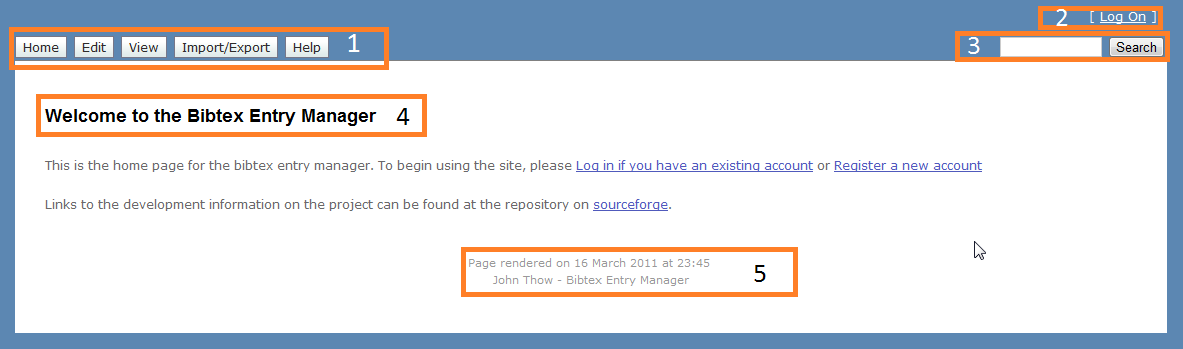
\includegraphics
			[scale=0.5]
			{images/PageLayout.png}
		\caption{Annotation of a page}
		\label{fig:pageLayout}
	\end{center}
\end{figure}

\begin{figure}
	\begin{center}
		
\includegraphics
			{images/LogOff.png}
		\caption{The log on area when a user is logged in (swapped out for area 2 in figure \ref{fig:pageLayout})}
		\label{fig:logOff}
	\end{center}
\end{figure}

\begin{enumerate}
	\item Firstly, there is a menu area which appears on every page within the site, with the same options at each appearance.  This gives the user a single point of reference to aid navigation of the website \revisit - cite someone
	\item The log on area appears in one of two forms across all pages of the application: a user is either browsing anonymously, or is logged in.  It is clear which of these two states the user's session is in thanks to the clear representation of the words `Log On' (depicted in figure \ref{fig:pageLayout}) and a welcome message with the current user's email address (as depicted in figure \ref{fig:logOff})
	\item After feedback from a user during the basic evaluation (see Chapter \ref{eval}) the interface was updated to include a search area on all pages.  The provision of this area allows a user to efficiently search the system's database for a string and, by making it a consistent feature, gives another concrete point of reference across all pages.
	\item Each and every page contains a bold header indicating the title of the page.  The presence of a title on each page gives a user another concrete and consistent place to glance in order to gain an insight into what they previously clicked on, as well as giving confirmation that their previous action was successful.
	\item The fifth item highlighted in this image provides some extra, arguably unnecessary information.  The main idea behind including this page render time area is to provide extra feedback: it lets a user know that page has finished loading, that it has been completed successfully and it reassures a user that the page is up to date.
\end{enumerate}

This consistency was implemented using a feature in \gls{asp}.\gls{net} called Master Pages.  As the name suggests, the developer creates a master page with the main layout of the website, within which sit containers which are filled by individual pages.  This approach centralises the code for the pages, the advantages and disadvantages of this are discussed in section \ref{codeReuse}. \revisit revisit fluency.

The colour choice of the interface was a decision which was postponed until later in the project, so that the bulk of the development work could be carried out before aesthetics were considered.  The colour scheme seen in the project is heavily based on the default style for projects created in \gls{msvs} 2010; it soon became apparent that the default style had many strong qualities that could be used 

\section{Concurrency}
Possible approaches:\\
Pessimistic: Lock users out while one works on it \\
Optimistic: Allow all to view/delete/amend and notify when others have performed actions\\
No concurrency control, real-time updates instead